% FONTE TEMA https://github.com/matze/mtheme
\documentclass[aspectratio=1610]{beamer}
%\documentclass[aspectratio=1610, handout]{beamer}
\usepackage[utf8]{inputenc}
\usepackage{ragged2e}
\usepackage{xcolor}
\usepackage[italian]{babel}
\usepackage{multirow}
\usepackage{silence}
\WarningFilter{beamer}{}
\WarningFilter{metropolis}{}
\usetheme[progressbar=frametitle,titleformat=smallcaps]{metropolis}
\setbeamertemplate{frame numbering}[fraction]
\setbeamercovered{dynamic}
\definecolor{rosso}{RGB}{255, 0, 0}
\definecolor{giallo}{RGB}{254,212,23}
\hypersetup{colorlinks=true,linkcolor=black,urlcolor=rosso}
\setbeamercolor{palette primary}{fg=black, bg=giallo}
\setbeamercolor{background canvas}{bg=white}
\setbeamercolor{normal text}{fg=black}
\setbeamercolor{progress bar}{fg=rosso}
\setbeamercolor{framesubtitle}{fg=rosso}
\setbeamercolor{normal text .dimmed}{fg=giallo}
\setbeamercolor{block title alerted}{fg=rosso, bg=giallo}
\setbeamerfont{caption}{size=\tiny}
\setbeamerfont{caption name}{size=\tiny}
\setlength{\abovecaptionskip}{0pt}
\makeatletter
\metroset{block=fill}
\setlength{\metropolis@progressinheadfoot@linewidth}{1pt} 
\setlength{\metropolis@progressonsectionpage@linewidth}{1pt}
\setlength{\metropolis@titleseparator@linewidth}{1pt}
\makeatother

\title{PROGETTAZIONE DI UNA BASE DI DATI}
\subtitle{Schema concettuale (E/R)}
\date{}
\institute{\textit{
        Fonti:
        \begin{itemize}
            \item[-] \href{https://catalogo.sanoma.it/si-op-104157-dal-bit-all-intelligenza-artificiale.html\#bundles.tab}{Dal Bit all'Intelligenza Artificiale}
            \item[-] \href{https://it.wikipedia.org/wiki/Modello_E-R}{Wikipedia}
        \end{itemize}
    }
}

\begin{document}

\begin{frame}[plain, noframenumbering]
    \titlepage
\end{frame}

\begin{frame}{MODELLO ER}
    \begin{alertblock}{DEFINIZIONE}
        \begin{minipage}{0.98\linewidth}
            \justifying
            Il modello \textbf{ER} concettuale (\textbf{E}ntity-\textbf{R}elationship) è un linguaggio 
            di modellazione utilizzato per rappresentare le strutture dei dati 
            in un database. È un approccio visivo per descrivere la struttura 
            dei dati e le relazioni tra essi.\\
            \bigskip
        \end{minipage}
    \end{alertblock}
\end{frame}

\section{COMPONENTI PRINCIPALI}

\begin{frame}{COMPONENTI PRINCIPALI}
    \begin{columns}
        \column{.5\textwidth}
            \begin{alertblock}{ENTIT\'A}
                \begin{minipage}{0.96\linewidth}
                    \justifying
                    Rappresenta una classe di oggetti o un elemento del dominio di 
                    interesse, come ad esempio "Cliente", "Ordine" o "Prodotto". 
                    Ogni entità è caratterizzata da un nome univoco all’interno della base di dati.\\
                    \bigskip
                \end{minipage}
            \end{alertblock}
        \column{.5\textwidth}
            \begin{figure}
                \includegraphics[width=\linewidth]{img/entità.png}
                \caption{{creata con \href{www.canva.com}{Canva}}}
            \end{figure}
    \end{columns}
\end{frame}

\begin{frame}{COMPONENTI PRINCIPALI}
    \begin{columns}
        \column{.5\textwidth}
            \begin{alertblock}{ASSOCIAZIONE}
                \begin{minipage}{0.96\linewidth}
                    \justifying
                    Rappresenta la connessione tra due o più entità, come ad 
                    esempio "Un ordine è associato a un prodotto" o "Un personaggio 
                    affronta uno o più livelli". Ogni associazione è caratterizzata da un nome.\\
                    \bigskip
                \end{minipage}
            \end{alertblock}
        \column{.5\textwidth}
            \begin{figure}
                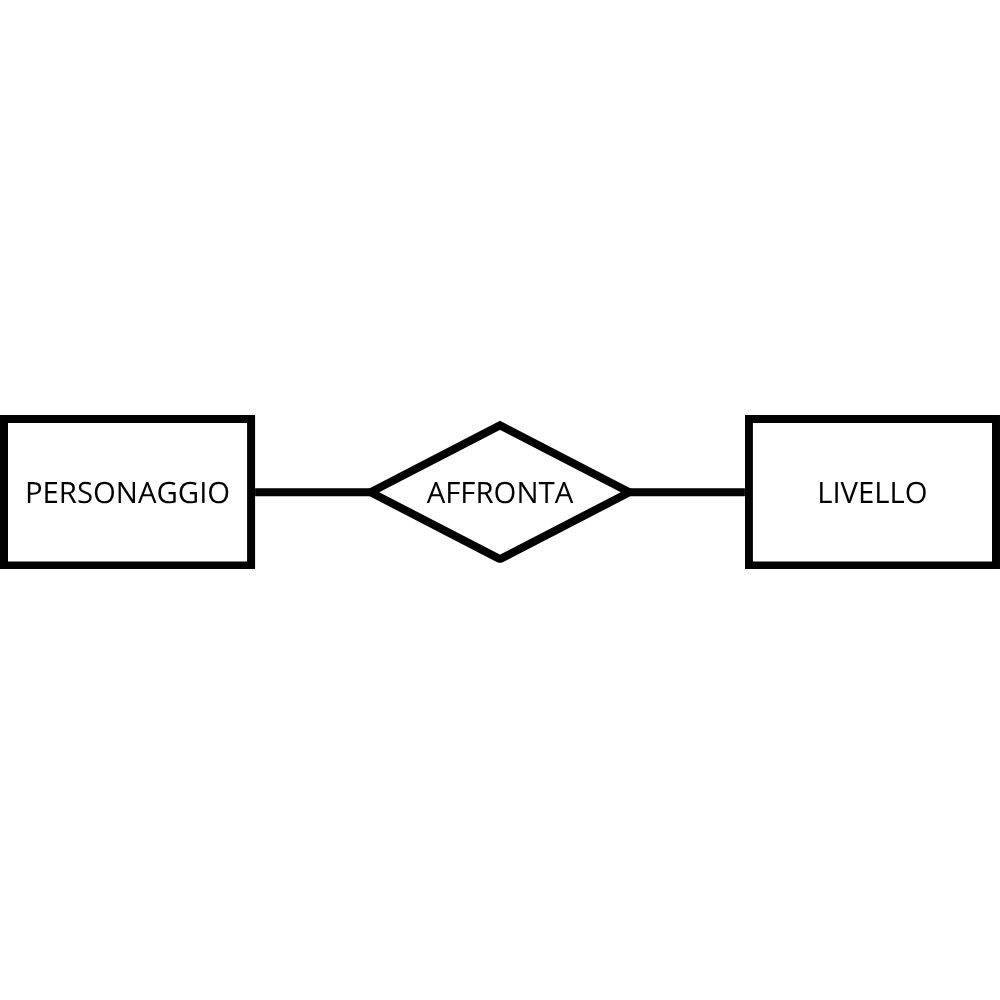
\includegraphics[width=\linewidth]{img/associazione.png}
                \caption{{creata con \href{www.canva.com}{Canva}}}
            \end{figure}
    \end{columns}
\end{frame}

\begin{frame}{COMPONENTI PRINCIPALI}
    \begin{columns}
        \column{.5\textwidth}
            \begin{alertblock}{ATTRIBUTO}
                \begin{minipage}{0.96\linewidth}
                    \justifying
                    Descrive una caratteristica di un’entità o di una associazione, 
                    come ad esempio un "nome", "cognome" o "prezzo". Ogni 
                    attributo è caratterizzato da un nome univoco all’interno dell’entità considerata.\\
                    \bigskip
                \end{minipage}
            \end{alertblock}
        \column{.5\textwidth}
            \begin{figure}
                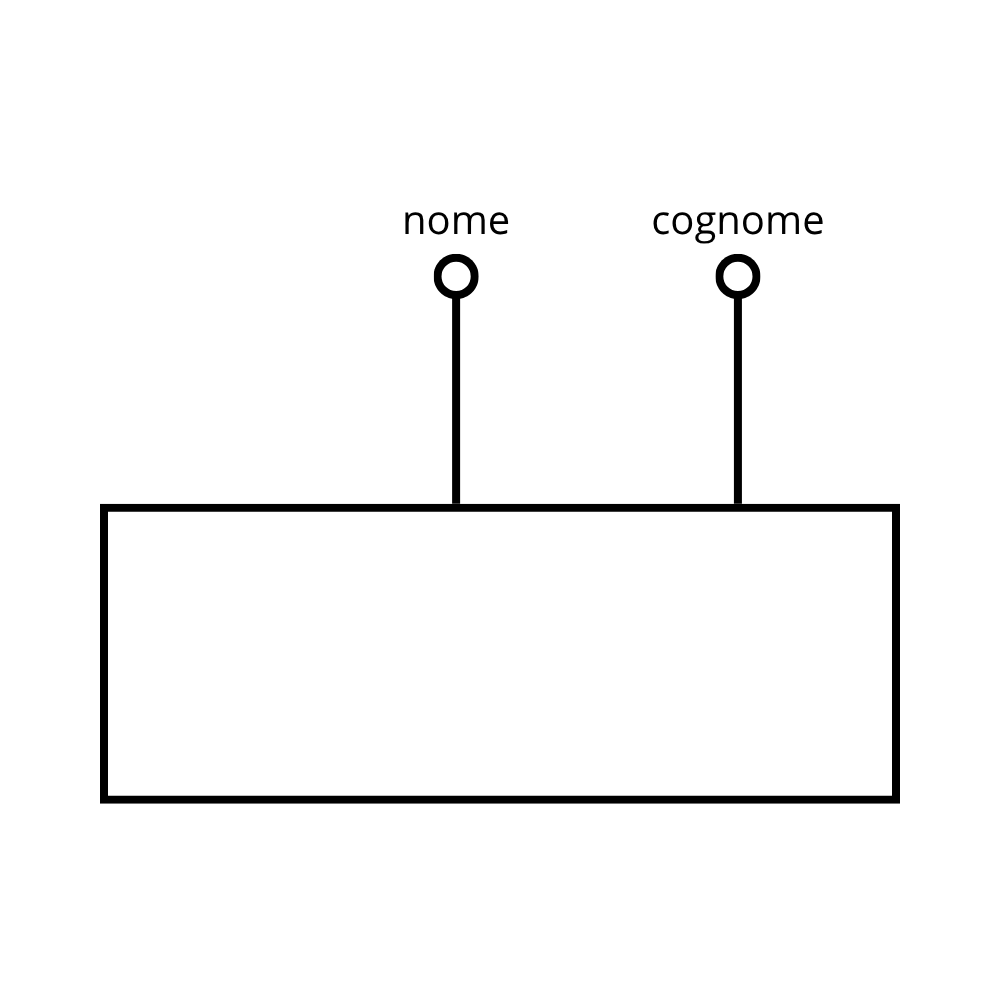
\includegraphics[width=\linewidth]{img/attributo.png}
                \caption{{creata con \href{www.canva.com}{Canva}}}
            \end{figure}
    \end{columns}
\end{frame}

\section{TIPOLOGIE DI ASSOCIAZIONE}

\begin{frame}{CARDINALIT\'A}
    \begin{alertblock}{DEFINIZIONE}
        \begin{minipage}{0.98\linewidth}
            \justifying
            La cardinalità di una associazione rappresenta la quantità di 
            entità che possono essere associate a un'altra entità in una 
            associazione. In altre parole, indica quanti elementi di una entità 
            possono essere collegati a un elemento di un'altra entità.\\
            \pause
            La cardinalità è definita dalla coppia \textbf{(cardinalità minima, cardinalità massima)}.\\
            La \textbf{cardinalità minima} può assumere i valori:
            \begin{itemize}
                \item \textbf{0} per indicare un’associazione opzionale;
                \item \textbf{1} per indicare un’associazione obbligatoria.
            \end{itemize}
            La \textbf{cardinalità massima} può assumere i valori:
            \begin{itemize}
                \item \textbf{1} (uno);
                \item \textbf{N} (molti).
            \end{itemize}
        \end{minipage}
    \end{alertblock}
\end{frame}

\begin{frame}{TIPOLOGIE DI ASSOCIAZIONE}
    \begin{figure}
        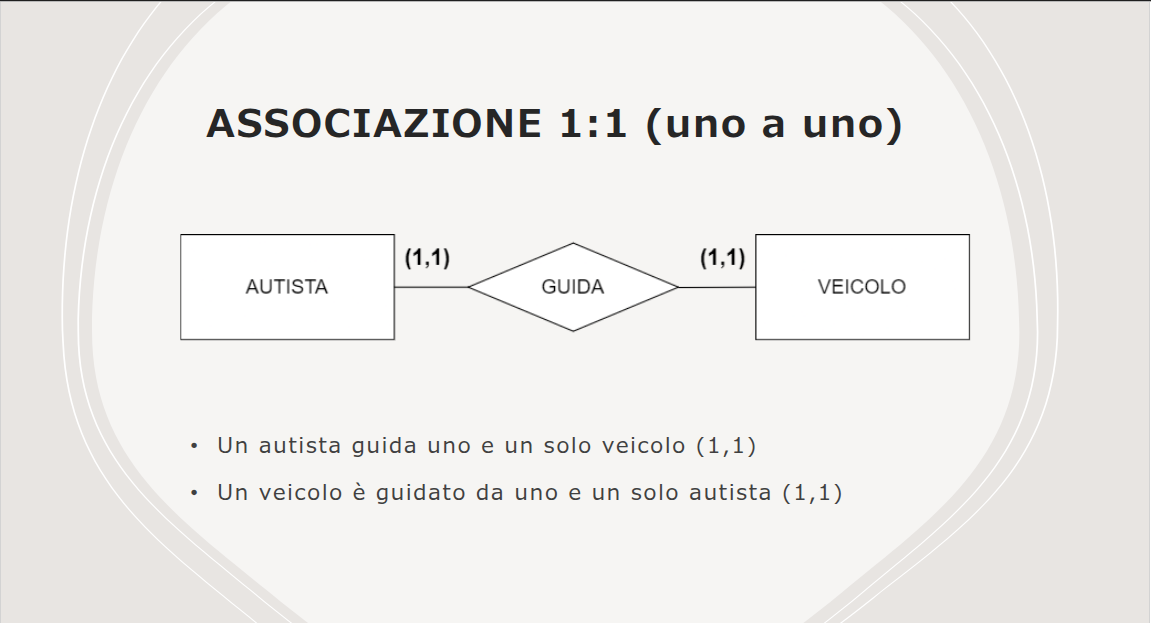
\includegraphics[width=\linewidth]{img/1a1.png}
        \caption{{creata con \href{https://docs.google.com/presentation/}{Google Slides}}}
    \end{figure}
\end{frame}

\begin{frame}{TIPOLOGIE DI ASSOCIAZIONE}
    \begin{figure}
        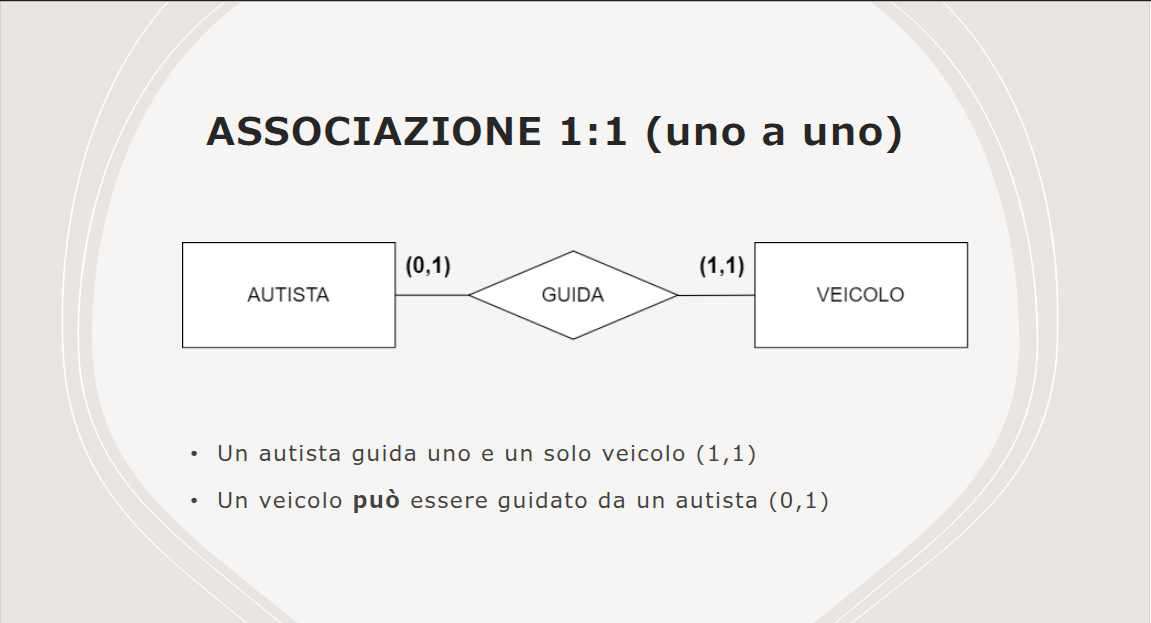
\includegraphics[width=\linewidth]{img/1a1_2.png}
        \caption{{creata con \href{https://docs.google.com/presentation/}{Google Slides}}}
    \end{figure}
\end{frame}

\begin{frame}{TIPOLOGIE DI ASSOCIAZIONE}
    \begin{figure}
        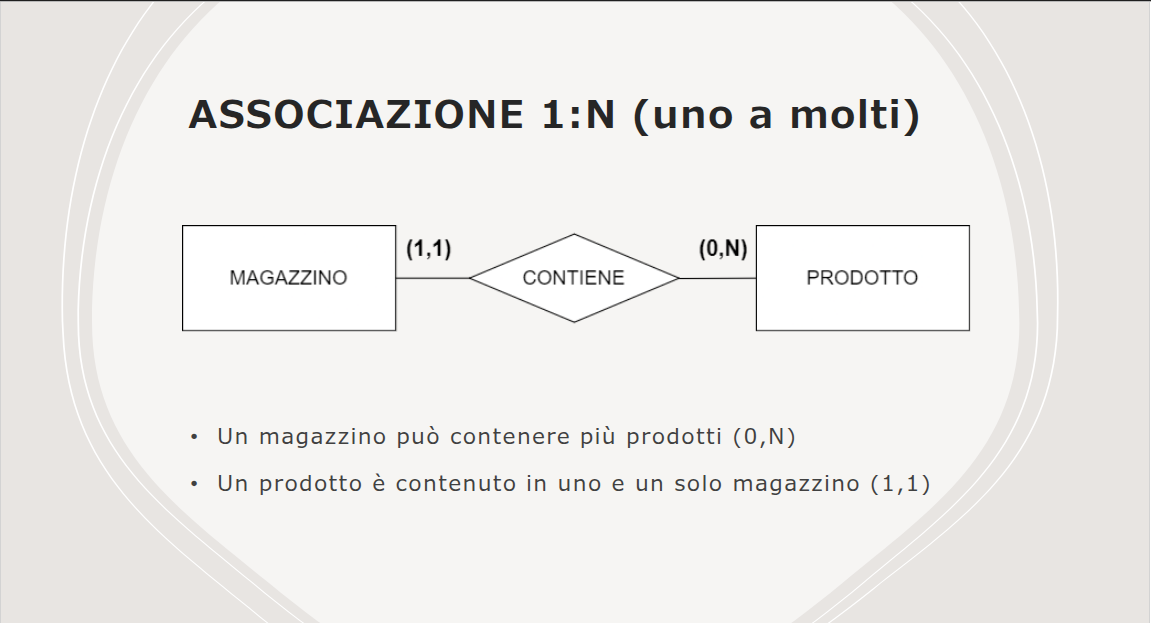
\includegraphics[width=\linewidth]{img/1an.png}
        \caption{{creata con \href{https://docs.google.com/presentation/}{Google Slides}}}
    \end{figure}
\end{frame}

\begin{frame}{TIPOLOGIE DI ASSOCIAZIONE}
    \begin{figure}
        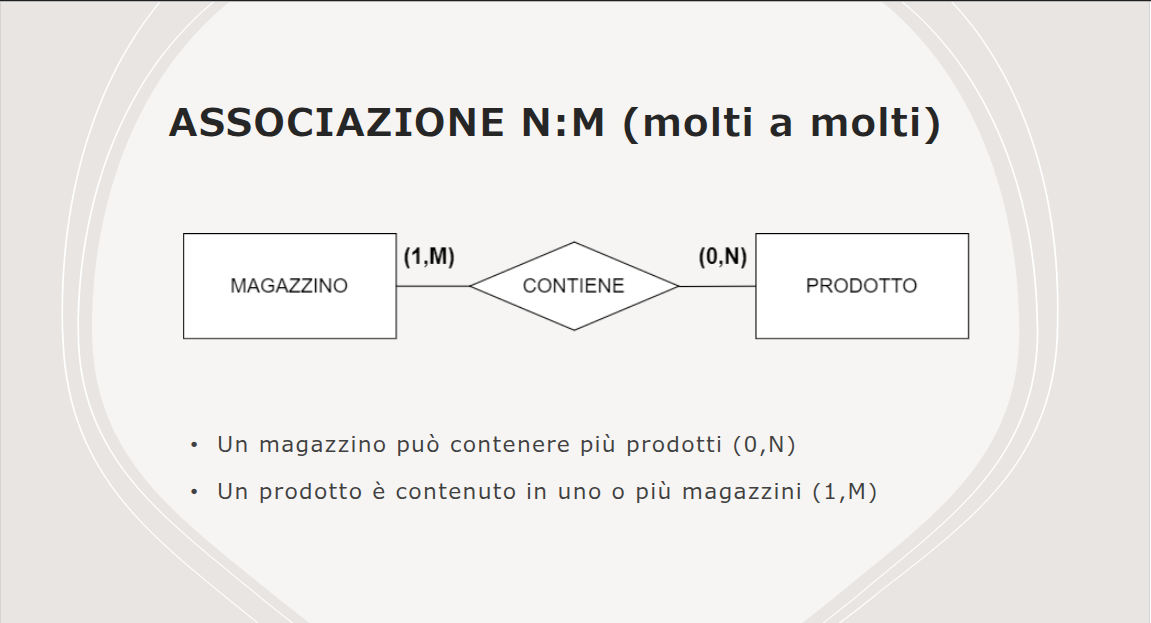
\includegraphics[width=\linewidth]{img/nam.png}
        \caption{{creata con \href{https://docs.google.com/presentation/}{Google Slides}}}
    \end{figure}
\end{frame}

\section{TIPOLOGIE DI ATTRIBUTO}

\begin{frame}{TIPOLOGIE DI ATTRIBUTO}
    \begin{columns}
        \column{.5\textwidth}
            \begin{alertblock}{ATTRIBUTO SEMPLICE}
                \begin{minipage}{0.96\linewidth}
                    \justifying
                    Un attributo viene definito semplice quando contiene uno e un solo valore. \\
                    \bigskip
                \end{minipage}
            \end{alertblock}
        \column{.5\textwidth}
            \begin{figure}
                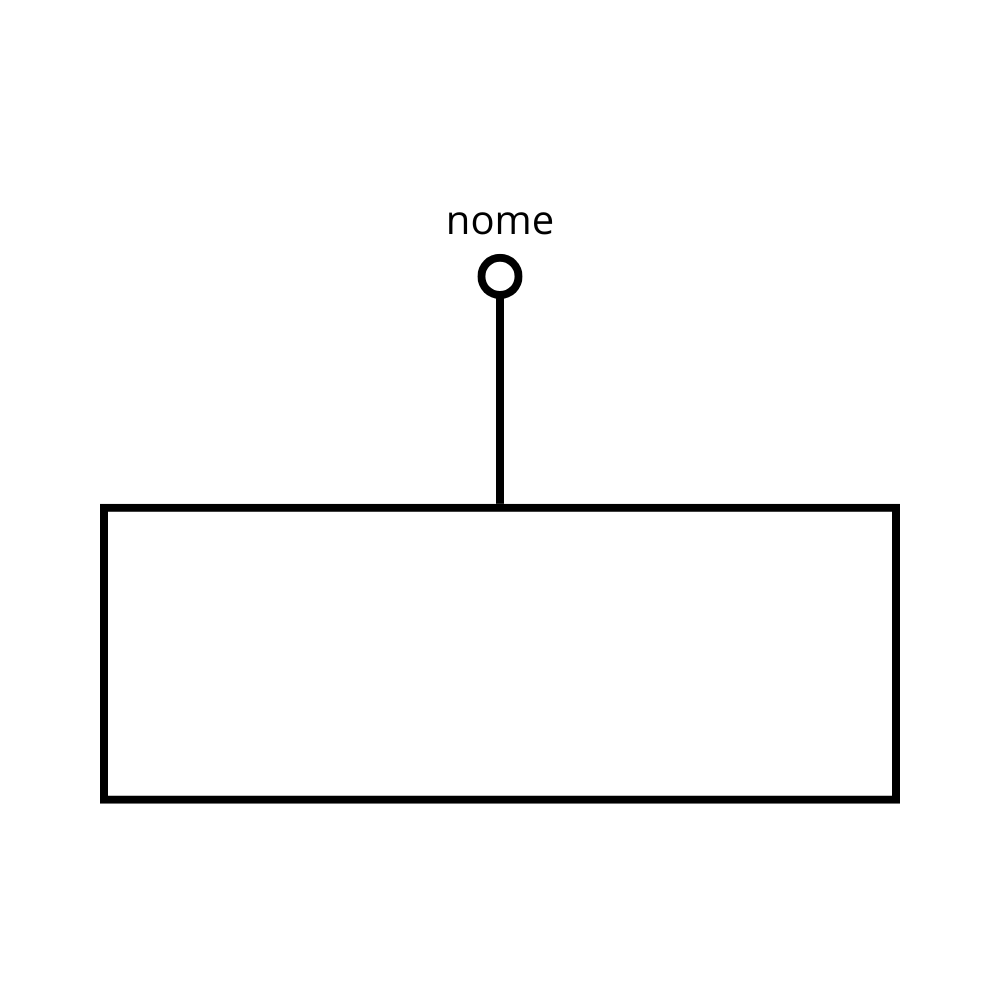
\includegraphics[width=\linewidth]{img/attributo_semplice.png}
                \caption{{creata con \href{www.canva.com}{Canva}}}
            \end{figure}
    \end{columns}
\end{frame}

\begin{frame}{TIPOLOGIE DI ATTRIBUTO}
    \begin{columns}
        \column{.5\textwidth}
            \begin{alertblock}{ATTRIBUTO SEMPLICE}
                \begin{minipage}{0.96\linewidth}
                    \justifying
                    Un attributo viene definito semplice quando contiene uno e un solo valore. 
                    Anche le associazioni posso avere attributi.\\
                    \bigskip
                \end{minipage}
            \end{alertblock}
        \column{.5\textwidth}
            \begin{figure}
                
\includegraphics[width=\linewidth]{img/attributo_associazione.png}
                \caption{{creata con \href{www.canva.com}{Canva}}}
            \end{figure}
    \end{columns}
\end{frame}

\begin{frame}{TIPOLOGIE DI ATTRIBUTO}
    \begin{columns}
        \column{.5\textwidth}
            \begin{alertblock}{ATTRIBUTO OPZIONALE}
                \begin{minipage}{0.96\linewidth}
                    \justifying
                    Un attributo viene definito opzionale quando è ammessa l’assenza del 
                    valore dell’attributo.\\
                    \bigskip
                \end{minipage}
            \end{alertblock}
        \column{.5\textwidth}
            \begin{figure}
                
\includegraphics[width=\linewidth]{img/attributo_opzionale.png}
                \caption{{creata con \href{www.canva.com}{Canva}}}
            \end{figure}
    \end{columns}
\end{frame}

\begin{frame}{TIPOLOGIE DI ATTRIBUTO}
    \begin{columns}
        \column{.5\textwidth}
            \begin{alertblock}{ATTRIBUTO COMPOSTO}
                \begin{minipage}{0.96\linewidth}
                    \justifying
                    Un attributo viene definito composto quando è definito come l’aggregazione 
                    di molteplici valori. Ad esempio: data (gg, mm, aaaa) o indirizzo (toponimo, 
                    nome, numero civico).\\
                    \bigskip
                \end{minipage}
            \end{alertblock}
        \column{.5\textwidth}
            \begin{figure}
                
\includegraphics[width=\linewidth]{img/attributo_composto.png}
                \caption{{creata con \href{www.canva.com}{Canva}}}
            \end{figure}
    \end{columns}
\end{frame}

\begin{frame}{TIPOLOGIE DI ATTRIBUTO}
    \begin{columns}
        \column{.5\textwidth}
            \begin{alertblock}{IDENTIFICATORE NATURALE}
                \begin{minipage}{0.96\linewidth}
                    \justifying
                    Un identificatore è un attributo (o un insieme di attributi) che caratterizza 
                    in modo univoco ciascuna singola istanza di un’entità. In altri termini, 
                    non possono esserci due istanze di una stessa entità le quali abbiano lo 
                    stesso identificatore.\\
                    \bigskip
                \end{minipage}
            \end{alertblock}
        \column{.5\textwidth}
            \begin{figure}
                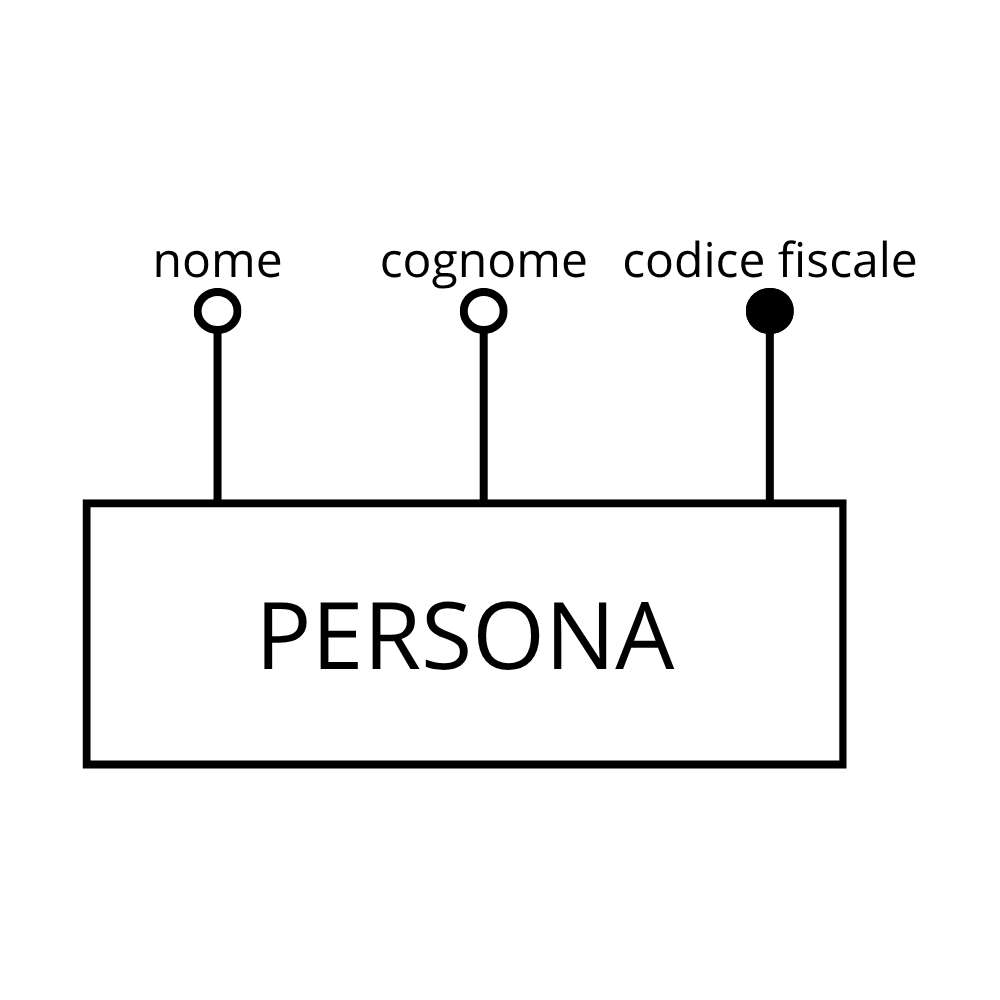
\includegraphics[width=\linewidth]{img/id_naturale.png}
                \caption{{creata con \href{www.canva.com}{Canva}}}
            \end{figure}
    \end{columns}
\end{frame}

\begin{frame}{TIPOLOGIE DI ATTRIBUTO}
    \begin{columns}
        \column{.5\textwidth}
            \begin{alertblock}{DENTIFICATORE ARTIFICIALE}
                \begin{minipage}{0.96\linewidth}
                    \justifying
                    Un identificatore artificiale è un attributo: \textbf{ID}, che caratterizza in 
                    modo univoco ciascuna singola istanza di un’entità tramite un numero che 
                    incrementa per ogni singola istanza dell’entità. In altri termini, un numero 
                    di riga per ogni istanza. Si utilizza nel caso non sia possibile determinare un 
                    identificatore naturale.\\
                    \bigskip
                \end{minipage}
            \end{alertblock}
        \column{.5\textwidth}
            \begin{figure}
                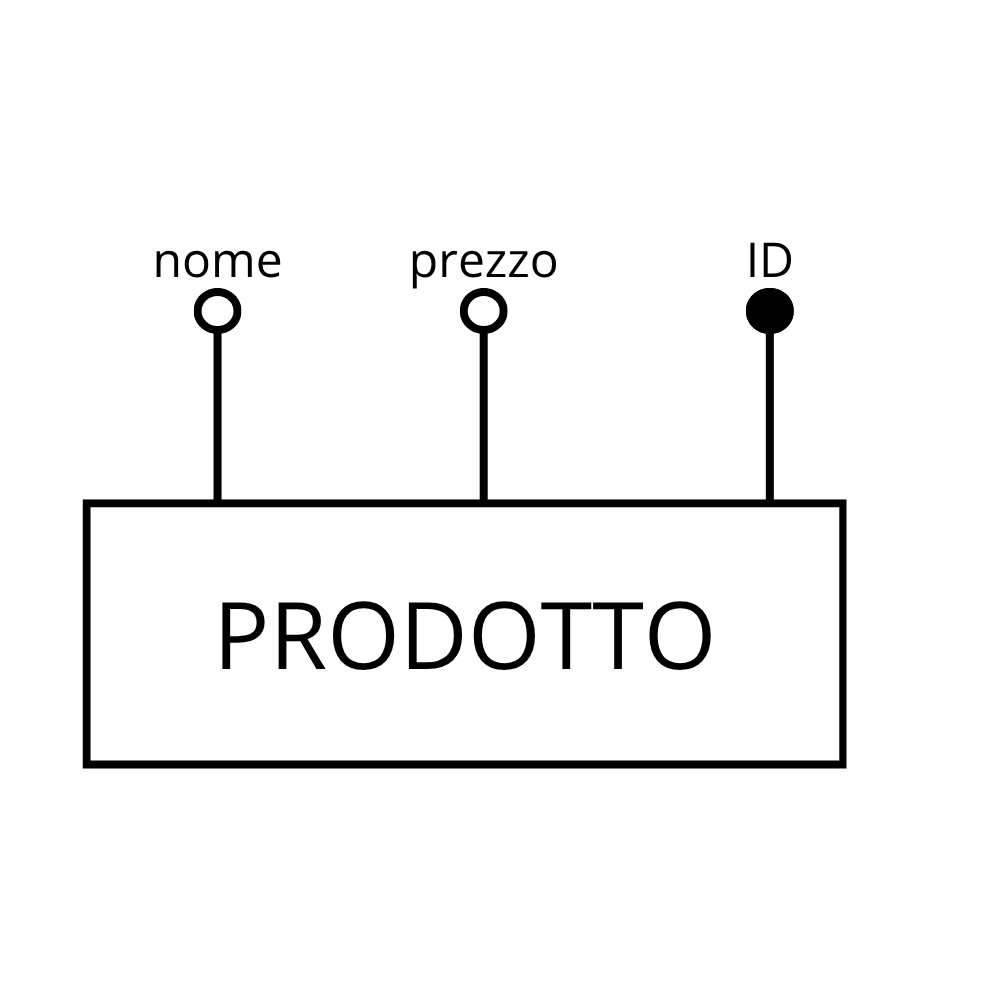
\includegraphics[width=\linewidth]{img/id_artificiale.png}
                \caption{{creata con \href{www.canva.com}{Canva}}}
            \end{figure}
    \end{columns}
\end{frame}

\end{document}